\section{How and What to Test}\label{sect:hwtest}
When developing a test framework it is important to ask, what testers would like to test and how they would like to perform testing. To make the framework natural to use, we want to reuse ideas common testing concepts. So even though we focus on testing on the system level, we will take some cues from the unittest package in python. In this package, like with many unit testing frameworks, testing is structured into test cases and suites. A test case is an assertion about the program. An example could be that we assert function foo() to return True.  A suite is a collection of test cases. It also contains some setup code.  For our framework the suite setup code runs the ETL system on a set of test sources and a DW supplied by the tester. The suite’s test cases are then run upon the DW resulting from the ETL run. Thus our test cases can be described as assertions about a given DW.  

What assertions do we then want to be able to make about a DW?  To better define our framework we decide that it should be used for source to target testing. This is a type of validation testing taking place after a load, where we test whether the data in the DW is what we expect it to be. As such the framework is delimited from areas of testing concerning performance and security. It is wholly data centered. Even then, it is difficult to define what to focus on in such a test. The literature contains many different suggestion on what to test.  In the following subsections we dicuss, what we deem to be the most important areas of testing.

\subsection{Data integrity}
For a DW to be useful we want there to be data integrity. That is, stored data is both  accurate and consistent. 3 rules ensure data integrity:  

\begin{itemize}
\item Entity integrity
\item Referential integrity
\item Domain integrity
\end{itemize}

Entity integrity concerns primary keys. It states that every table should have a primary key and that it should be unique and not null for each entry. Referential integrity is about foreign keys. It enforces that a foreign key should either refer to the primary key of another table or be null. This means that a foreign key can not refer to a primary key that does not exist.  Domain integrity relates to the values taken on by attributes. It says that all attributes must have a defined domain. Likewise the values of attributes in all tuples should stay within their defined domain. Data integrity is important as it allows us to assert certain truths about our database. Such as each tuple in a table being identifiable or that a join between two tables is possible. Despite these advantages, DBMS' may not enforce them during loads. Loading data into a DW using an ETL usually involves a large amount of data and access to the DW is shut down temporarily. Checking each entry for data integrity can be expensive. Therefore a fast load often takes precedence over a safe load. If the ETL system is improperly designed, the DW ends up not having data integrity, which may hinder its usefulness. If the framework can assist in testing for data integrity, we can ensure future data integrity.

\subsection{Data Loss}
Through the ETL process, data from sources makes its way into a DW. This new data contains information relevant to future business analysis performed by users. However, information may get lost during the process. Data loss may occur in any of the three subprocesses. It is possible that the wrong data is extracted from the sources. Transformations may be faulty and produce an incorrect result. Loss during load may occur  through truncation. Truncation occurs, when the datatype of a DW attribute cannot store the amount of data necessary. This often results in the data being cut to fit the data type, and thus data is lost.  The result of any data loss is a DW not containing the needed information. This leads to poor business analysis. The framework should assist in ensuring that no data loss occurs during the process.

\subsection{Business Rules}
The term business rule is generally used for all rules applied to data stored in a database. This also includes data integrity as spoken about before. However data integrity could be seen as an ideal from which the business rules may differ. In the case of DWs the actual business rules often do not enforce entity integrity upon the fact table as the access of a specific entry may be unnecessary. Business rules however do not only pertain to data integrity as it is a rather broad term. An example of this could be an attribute relationships such as hierarchies. Another type of business rule could describe the schema of a specific table.

\begin{figure}
  \centering
		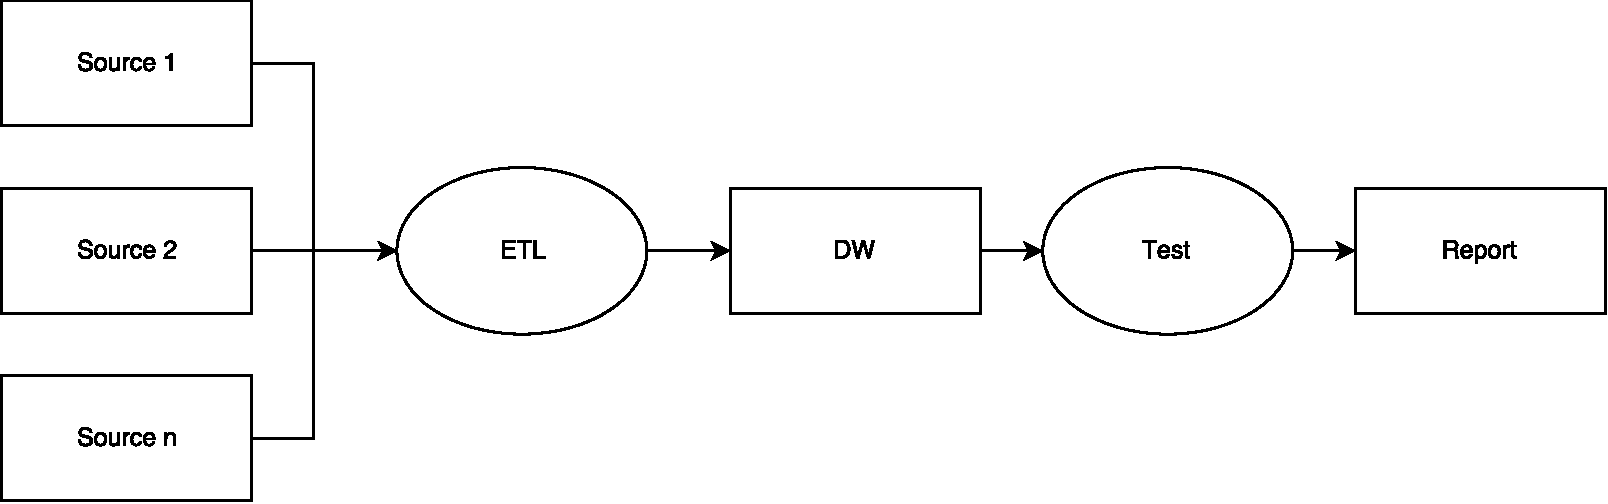
\includegraphics[width=0.5\textwidth]{figures/scenario.pdf}
  \caption{Diagram of source to target test}
	\label{fig:sourcetotarget}
\end{figure}

%%Men skal det ligger her? Jeg er ikke sikker.

\subsection{Source to Target Test}
The purpose of a source to target test is to find errors in the ETL process. If we know what the sources look like, as well as how the transformations should perform, we can make general assertions on how the resulting DW should look. When we make assertions on the DW that is the result of the ETL process,  we may refer to this as a source to target test, see Figure \ref{fig:sourcetotarget}. This kind of test can be wide and include many small to big test cases, and may thus be expensive to execute on large DWs. Note that a DW that is in use by a business, may have had its transformations re-factored due to changes to business rules. This means that our assertions about the current implementation could fail even though they are correct. Thus this kind of test should focus on smaller sources, that transform into a fresh DW that is then easy and fast to conduct tests on. These sources in turn would preferably be set up as mock sources rather than large business sources. The results of such tests should give information on how the transformations perform according to specification and in turn help lower the risk of the ETL program.






